\documentclass[a4paper]{ltjsarticle}

% LuaTeX
\usepackage{luatexja-fontspec}
\usepackage[no-math,match,deluxe,sourcehan-jp]{luatexja-preset}

% 基本パッケージ
\usepackage{graphicx}
\usepackage[svgnames]{xcolor}
\usepackage{here}
\usepackage{amsmath, amssymb, amsthm}
\usepackage{mathtools}
\usepackage[unicode,hidelinks,pdfusetitle]{hyperref}
\usepackage{nameref}
\usepackage{cleveref}
\usepackage{comment}

% 追加パッケージ
\usepackage[ISO]{diffcoeff}
\usepackage{enumitem}
\usepackage{tikz}
\usepackage{tcolorbox}

% パッケージのライブラリ
\usetikzlibrary{datavisualization.formats.functions}
\tcbuselibrary{breakable,skins,theorems}

% メタデータ
\title{補間多項式による数値計算}
\author{cuttlefish\_math}
\date{\today}

% レイアウト操作
\setsansjfont[BoldFont=Source Han Sans JP Medium]{Source Han Sans JP}
\renewcommand{\kanjifamilydefault}{\gtdefault}

% 参照
\crefname{theorem}{定理}{定理}
\crefname{definition}{定義}{定義}
\crefname{example}{例}{例}
\crefname{lemma}{補題}{補題}
\crefname{subsection}{節}{節}

% 定理環境
\theoremstyle{definition}

\tcbset{%
  mystyle/.style={%
    enhanced,
    label type={#1},
    theorem style=plain,
    fonttitle=\bfseries,
    colframe=black,
    colback=white,
    colbacktitle=white,
    coltitle=black,
    enlarge top by=0.6\zh,
    arc=0mm,
    boxrule=0.2mm}}

\newtcbtheorem[number within=section]{theorem}{定理}{mystyle={theorem}}{theorem}
\newtcbtheorem[number within=section]{definition}{定義}{mystyle={definition}}{definition}
\newtcbtheorem[number within=section]{lemma}{補題}{mystyle={lemma}}{lemma}
\newtheorem{example}{例}[section]

% マクロ定義
\DeclarePairedDelimiter{\abs}{\lvert}{\rvert}
\DeclarePairedDelimiter{\pqty}{\lparen}{\rparen}
\DeclarePairedDelimiter{\bqty}{\lbrack}{\rbrack}

\newcommand{\dd}[1]{\dl2#1}
\newcommand{\plimas}[1]{\pod{#1}}
\newcommand{\degree}[1]{{#1}^\circ}
\newcommand{\zahl}{\mathbb{Z}}

\begin{document}
\maketitle
\tableofcontents

\section{はじめに}
計算機上で関数を扱うには,関数をよく知られた扱いやすい関数で近似できると何かと便利である.
中でも扱いやすい関数は多項式関数であろう.$+$と$\times$の2つの演算さえ実行できれば計算でき,
しかも,曲線として表現できる幅もそれなりに広い.本稿では,この多項式関数によって,種種の計算を近似的に行う方法を紹介する.

\section{補間多項式}
\subsection{ラグランジュ補間}
次の定理は,本稿を通して重要な役割を担うものである.

\begin{theorem}{補間多項式の一意存在性}{interpolation}
  実数の組$P_1 = (p_1, q_1), \dots, P_n = (p_n, q_n)$は,$i \neq j$なら必ず$p_i \neq p_j$を満たすとする.
  このとき,任意の$i = 1,\dots,n$について変数$x$に$p_i$を代入した値が$q_i$であり,かつ次数が$n-1$以下である多項式$f(x)$がただ1つ存在する.
\end{theorem}

\begin{proof}
  まず存在性を示す.$i=1,\dots,n$に対し,多項式$g_i(x)$を
  \[
    g_i(x) = (x-p_1) \cdots (x-p_{i-1})(x-p_{i+1}) \cdots (x-p_n)
  \]
  で定義する.このとき
  \[
    g_i(p_j) = {
      \begin{cases}
        (p_j-p_1) \cdots (p_j-p_{i-1})(p_j-p_{i+1}) \cdots (p_j-p_n) & (j = i) \\
        0 & (j \neq i)
      \end{cases}
      \quad
      (j = 1,\dots,n)
    }
  \]
  である.仮定により$i \neq j$なら$p_i \neq p_j$なので,$g_i (p_i) \neq 0$である.したがって
  \[
    f(x) = q_1h_1(x) + \cdots + q_nh_n(x),
    \quad
    h_i(x) = \frac{1}{g_i(p_i)} g_i(x)
  \]
  により多項式$f(x), h_1(x), \dots, h_n(x)$を定義すれば
  \begin{align*}
    f(p_i)
    &= q_1h_1(p_i) + \cdots + q_nh_n(p_i) \\
    &= q_10 + \cdots + q_{i-1}0 + q_i\pqty*{\frac{1}{g_i(p_i)} g_i(p_i)} + q_{i+1}0 + \cdots + q_n0 \\
    &= q_i
  \end{align*}
  となる.$h_1(x), \dots, h_n(x)$の次数は$n-1$次なので,これらの定数倍の和である$f(x)$の次数は最大でも$n-1$である.

  次に一意性を示す.多項式$f_1(x), f_2(x)$はともに次数が$n-1$以下であり,かつすべての$i = 1, \dots, n$に対して$q_i = f_1(p_i) = f_2(p_i)$を満たすとする.
  $g(x) = f_1(x) - f_2(x)$で多項式$g(x)$を定義すると,$g(x)$の次数も$n-1$以下である.
  また,$x = p_1, \dots, p_n$のとき$g(x) = 0$であり,$p_1,\dots,p_n$はどの2つも相異なるので,因数定理により$g(x)$は$x-p_1,\dots,x-p_n$を因数に持つ.
  すなわち,$g(x)$は多項式$A(x)$によって
  \[
    g(x) = A(x)(x-p_1) \cdots (x-p_n)
  \]
  と書ける.$g(x)$の次数は$n-1$以下なので,この等式が成り立つには$A(x) = 0$でなければならない.よって$g(x) = 0$であるので,$f_1(x) = f_2(x)$が示された.
\end{proof}

\begin{definition}{ラグランジュの補間多項式}{lagrange}
  \cref{theorem:interpolation}の多項式$f(x)$をラグランジュの補間多項式(あるいは単に補間多項式)という.
  $f(x)$は次のように表せる{\footnotemark}.
  \[
    f(x) = \sum_{i=1}^n q_i \prod_{k\neq i} \frac{x - p_k}{p_i - p_k}
  \]
\end{definition}
\footnotetext{$\prod$は総乗記号であり,$\sum$の$+$を$\times$に置き換えたものである.この場合は$k=1,\dots,i-1,i+1,\dots,n$について積をとる.}

\begin{example}[補間多項式の例1]
  \label{example:lagrange_1}
  $(p_1,q_1)=(1,4),(p_2,q_2)=(3,0),(p_3,q_3)=(4,1)$のとき,補間多項式は
  \[
    f(x)
    = 4\cdot\frac{(x-3)(x-4)}{(1-3)(1-4)} + 0\cdot\frac{(x-1)(x-4)}{(3-1)(3-4)} + 1\cdot\frac{(x-1)(x-3)}{(4-1)(4-3)}
    = x^2-6x+9
  \]
  である.
\end{example}

\begin{example}[補間多項式の例2]
  \label{example:lagrange_2}
  $(p_1,q_1)=(1,6),(p_2,q_2)=(5,2),(p_3,q_3)=(4,3)$のとき,補間多項式は
  \[
    f(x)
    = 6\cdot\frac{(x-5)(x-4)}{(1-5)(1-4)} + 2\cdot\frac{(x-1)(x-4)}{(5-1)(5-4)} + 3\cdot\frac{(x-1)(x-5)}{(4-1)(4-5)}
    = -x+7
  \]
  である.このように,$n$個の点に関する補間多項式の次数は必ずしも$n-1$にならない.
\end{example}

\begin{figure}[H]
  \centering
  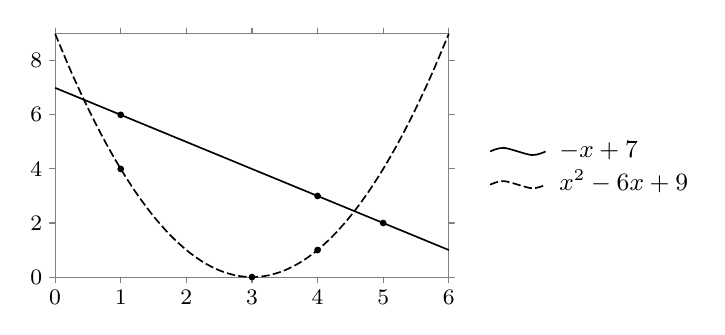
\begin{tikzpicture}
    \datavisualization [%
      scientific axes,
      visualize as smooth line/.list={deg1, deg2},
      visualize as scatter/.list={pts1, pts2},
      legend=east outside,
      pts1={style={mark=*, mark size=1pt}},
      pts2={style={mark=*, mark size=1pt}},
      deg1={label in legend={text=$-x+7$}},
      deg2={label in legend={text=$x^2-6x+9$}},
      style sheet=vary dashing
    ]
    data [set=deg1, format=function] {
      var x : interval [0:6];
      func y = -(\value x) + 7;
    }
    data [set=deg2, format=function] {
      var x : interval [0:6];
      func y = (\value x)^2 -6 * (\value x) + 9;
    }
    data [set=pts1] {
      x, y
      1, 6
      5, 2
      4, 3
    }
    data [set=pts2] {
      x, y
      1, 4
      3, 0
      4, 1
    };
  \end{tikzpicture}
  \caption{点と補間多項式の関係}
\end{figure}

\subsection{ニュートン補間}

この節では,補間多項式が通るべき点を追加したとき,補間多項式はどう変化するか考える.

\cref{theorem:interpolation}の状況で,$k=1,\dots,n$に対して,点$P_1,\dots,P_k$に関する補間多項式を$f_k(x)$とする.
$g_k(x) = f_k(x) - f_{k-1}(x)$とおくと,$i = 1,\dots,k-1$について$g_k(p_i)=0$である.$g_k(x)$の次数は最大でも$k-1$なので,因数定理により
\[
  g_k(x) = A_{k-1}(x-p_1)\cdots (x-p_{k-1})
\]
を満たす実数$A_{k-1}$が存在する.

したがって
\begin{align*}
  f_n(x) - f_{n-1}(x) &= A_{n-1}(x-p_1)\cdots (x-p_{n-2})(x-p_{n-1}) \\
  f_{n-1}(x) - f_{n-2}(x) &= A_{n-2}(x-p_1)\cdots (x-p_{n-2}) \\
  &\vdots \\
  f_2(x) - f_1(x) &= A_1(x-p_1) \\
  f_1(x) &= q_1
\end{align*}
である.すべて足すことで
\[
  f(x) = f_n(x) = q_1 + \sum_{k=1}^{n-1} A_k(x-p_1)\cdots (x-p_k)
\]
を得る.以上により,\cref{definition:lagrange}の補間多項式$f(x)$は,$n-1$個の実数$A_1,\dots,A_{n-1}$により上のように表せることが分かる.
また,この式に現れる$\sum$を$k=l-1$までで打ち切った多項式は$f_l(x)$であり,点$P_1,\dots,P_l$に関する補間多項式になっている.
このことをまとめると次のようになる.

\begin{theorem}{}{weak_newton}
  \cref{theorem:interpolation}の状況で,任意の$l=1,\dots,n$について多項式
  \[
    q_1 + \sum_{k=1}^{l-1} A_k(x-p_1)\cdots (x-p_k)
  \]
  が点$P_1,\dots,P_l$に関する補間多項式となるような実数$A_1,\dots,A_{n-1}$が存在する.
\end{theorem}

あとは$A_1,\dots,A_{n-1}$が$P_1,\dots,P_n$を用いて具体的に書ければよい.差商はこの簡便な表記を与える.

\begin{definition}{差商}{divided_differences}
  \cref{theorem:interpolation}の状況で,差商$[q_1, \dots, q_n]$を次のように定義する.
  \begin{align*}
    &[q_1] = q_1\\
    &[q_1,\dots,q_k] = \frac{[q_1,\dots,q_{k-1}]-[q_2,\dots,q_k]}{p_1-p_k} \quad (k \geqq 2)
  \end{align*}

  関数$g(x)$が$q_1=f(p_1),\dots,q_n=f(p_n)$を満たす場合,$[q_1,\dots,q_n]$を$g[p_1,\dots,p_n]$とも表記する.
\end{definition}

\begin{example}[差商の例]
  \label{example:divided_differences}
  $(p_1,q_1)=(1,6),(p_2,q_2)=(5,2),(p_3,q_3)=(4,3)$のとき
  \[
    [q_1, q_2] = \frac{6-2}{1-5} = -1,\,
    [q_2, q_3] = \frac{2-3}{5-4} = -1,\,
    [q_1,q_2,q_3] = \frac{-1-(-1)}{1-4} = 0
  \]
  である.
\end{example}

\begin{theorem}{ニュートン補間}{newton}
  \cref{theorem:interpolation}の状況で,$f(x)$は次のように表せる.
  \[
    f(x) = q_1 + \sum_{k=1}^{n-1} [q_1,\dots,q_{k+1}] (x-p_1) \cdots (x-p_k)
  \]
\end{theorem}

\begin{proof}
  帰納法により示す.$n=1$のときは$f(x)=q_1$なので明らかに成り立つ.
  次に,$n-1$個以下の点に関する補間多項式について成立を仮定する.点$P_1,\dots,P_n$に関する補間多項式を$f(x)$とする.
  点$P_1, \dots, P_{n-1}$に関する補間多項式を$g(x)$,$P_2, \dots, P_n$に関する補間多項式を$h(x)$とおくと,多項式
  \[
     \frac{(x-p_1)h(x) - (x-p_n)g(x)}{p_n-p_1}
  \]
  は次数が$n-1$以下であり,かつ点$P_1,\dots,P_n$を通る.\cref{theorem:interpolation}により補間多項式は一意なので,これは補間多項式$f(x)$である.
  右辺の$n-1$次の項の係数($0$であることもある)は,帰納法の仮定により
  \[
    \frac{[q_2,\dots,q_n]-[q_1,\dots,q_{n-1}]}{p_n-p_1} = [q_1,\dots,q_n]
  \]
  である.\cref{theorem:weak_newton}により,$f(x)$は実数$A_1,\dots,A_{n-1}$によって
  \[
    f(x) = q_1 + \sum_{k=1}^{n-1} A_k(x-p_1)\cdots (x-p_k)
  \]
  と書けるが,この$n-1$次の項の係数は$A_{n-1}$であるので
  \[
    f(x) = \pqty*{q_1 + \sum_{k=1}^{n-2} A_k(x-p_1)\cdots (x-p_k)} + [q_1,\dots,q_n](x-p_1)\cdots (x-p_{n-1})
  \]
  である.上の第1項は$g(x)$に等しいので,帰納法の仮定により
  \begin{align*}
    f(x)
    &= \pqty*{q_1 + \sum_{k=1}^{n-2} [q_1,\dots,q_{k+1}](x-p_1)\cdots (x-p_k)} + [q_1,\dots,q_n](x-p_1)\cdots (x-p_{n-1}) \\
    &= q_1 + \sum_{k=1}^{n-1} [q_1,\dots,q_{k+1}](x-p_1)\cdots (x-p_k)
  \end{align*}
  である.よって,$n$個の点に関する補間多項式についても命題は成り立つ.
\end{proof}

このように,多項式$(x-p_1) \dots (x-p_k)\,(k=1,\dots,n-1)$の定数倍の和によって,点$P_1,\dots,P_n$に関する補間多項式を得る方法をニュートン補間という.

\begin{example}[ニュートン補間の例]
  \cref{example:divided_differences}により,点$(1,6),(5,2),(4,3)$に関する補間多項式は
  \[
    6+(-1)(x-1)+0(x-1)(x-5) = -x+7
  \]
  である.\cref{theorem:interpolation}からも分かるように,これは\cref{example:lagrange_2}と一致している.
\end{example}

\subsection{補間多項式による近似の誤差}

補間多項式はしばしば,関数を近似するために用いられる.この節では,補間多項式による近似がどの程度妥当であるか分析する方法について考察する.

$n$は$2$以上の整数とする.$f(x)$を関数とし,曲線$y=f(x)$上の点$P_1=(x_1, f(x_1)),\dots,P_n=(x_n, f(x_n))$は$x_1<\dots<x_n$を満たすとする.
点$P_1,\dots,P_n$に関する補間多項式を$p(x)$とおくと,
$f(x)$が十分に滑らかであれば,$x$が$x_1,\dots,x_n$に近いとき$f(x)$の値と$p(x)$の値はごく近いことが期待できる.
次の定理はこのことを保証するものである.

\begin{theorem}{補間多項式による近似の誤差}{lagrange_error}
  上の状況で,関数$f(x)$は$n$階微分可能であるとする.このとき,任意の$t\in (x_1,x_n)$に対し
  \[
    f(t)-p(t) = \frac{f^{(n)} (\xi)}{n!} (t-x_1)\cdots (t-x_n)
  \]
  を満たす$\xi \in (x_1, x_n)$が存在する.これにより,$\abs*{f^{(n)}(x)}$が区間$[x_1, x_n]$で最大値を持てば
  \[
    \abs*{f(t)-p(t)}
    \leqq \max_{x_1\leqq\xi\leqq x_n} \frac{\abs*{f^{(n)}(\xi)}}{n!} \abs*{(t-x_1)\cdots (t-x_n)}
    \leqq \max_{x_1\leqq\xi\leqq x_n} \frac{\abs*{f^{(n)}(\xi)}}{n!} (x_n-x_1)^n
  \]
  である.
\end{theorem}

この定理は次の補題から導かれる.

\begin{lemma}{}{zero_existance}
  閉区間$I=[a,b]$で定義された関数$g(x)$は$I$における$n+1$個の点で$0$であり,かつ$I$で$n$階微分可能であるとする.
  このとき$g^{(n)}(\xi) = 0$を満たす$\xi \in (a,b)$が存在する.
\end{lemma}

\begin{proof}
  どの2つも相異なる$n+1$個の実数$x_1,\dots,x_{n+1} \in I$について$g(x_1) = \cdots = g(x_{n+1}) =0$であるとする.
  $j=1,\dots,n$に対し,$I_{1,j}=[x_j,x_{j+1}], \mathring{I}_{1,j}=(x_j,x_{j+1})$とおく.
  関数$g(x)$は$I_{1,j}$で連続かつ$\mathring{I}_{1,j}$で微分可能なので,平均値の定理により
  \[
    g^{(1)}(\xi_{1j}) = \frac{g(x_j)-g(x_{j+1})}{x_j-x_{j+1}} = \frac{0-0}{x_j-x_{j+1}}=0
  \]
  を満たす$\xi_{1,j} \in \mathring{I}_{1,j}$が存在する.
  これにより,$n$個の実数$\xi_{1,1} < \dots < \xi_{1,n}$を$g^{(1)}(x)$の値が$0$であるように取れる.この$n$項数列を$\xi_1 = \{ \xi_{1,n} \}$とする.

  同様に,$j=1,\dots,n-1$に対して,$I_{2,j}=[\xi_{1,j},\xi_{1,j+1}], \mathring{I}_{2,j}=(\xi_{1,j},\xi_{1,j+1})$とおく.再び平均値の定理により
  \[
    g^{(2)}(\xi_{2,j}) = \frac{g^{(1)}(\xi_{1,j})-g^{(1)}(\xi_{1,j+1})}{\xi_{1,j}-\xi_{1,j+1}} = \frac{0-0}{\xi_{1,j}-\xi_{1,j+1}} = 0
  \]
  を満たす$\xi_{2,j} \in \mathring{I}_{2,j}$が存在する.$\xi_{2,1},\dots,\xi_{2,n-1}$により,さきほどと同様に$n-1$項数列$\xi_2 = \{ \xi_{2,n} \}$を定義する.

  以下,これを繰り返すことによって数列$\xi_3,\dots,\xi_n$を定義する.$\xi_j$は$n+1-j$項数列であり,その項に現れる任意の数$a$は$g^{(j)}(a)=0$を満たす.
  よって,特に$j=n$のとき$\xi_n$は項をただ1つもち,その項$\xi$は$g^{(n)}(\xi)=0$を満たす.
\end{proof}

以上の補題により,\cref{theorem:lagrange_error}は次のように証明される.

\begin{proof}
  $t=x_2,\dots,x_{n-1}$のときは$(t-x_1)\cdots (t-x_n)=0$であるから,$\xi$は区間$(x_1,x_n)$上の任意の値にしてよい(たとえば$\xi=(x_1+x_n)/2$とすればよい).
  そこで,$t$が$x_2,\dots,x_{n-1}$のいずれとも等しくない場合について示す.
  \[
    g(x) = f(x)-p(x)-a(x-x_1)\cdots (x-x_n)
  \]
  とおく.ただし$a$は$g(t)=0$であるように取る.すなわち
  \[
    a = \frac{f(t)-p(t)}{(t-x_1)\cdots (t-x_n)}
  \]
  とする.

  $x=x_1,\dots,x_n,t$のとき$g(x)=0$であり,かつ関数$g(x)$は仮定により$n$階微分可能である.
  よって,\cref{lemma:zero_existance}により$g^{(n)}(\xi)=0$を満たす$\xi\in (x_1,x_n)$が存在する.ここで
  \[
    g^{(n)}(\xi) = f^{(n)}(\xi)-p^{(n)}(\xi)-an! = 0\quad\therefore\, a = \frac{f^{(n)}(\xi)-p^{(n)}(\xi)}{n!}
  \]
  である.$p(x)$の次数は最大でも$n-1$なので$p^{(n)}(\xi)=0$であり
  \[
    a = \frac{f^{(n)}(\xi)}{n!}
    \quad\therefore\, f(t)-p(t)-\frac{f^{(n)}(\xi)}{n!}(t-x_1)\cdots (t-x_n) = g(t) = 0
  \]
  となる.したがって
  \[
    f(t)-p(t) = \frac{f^{(n)}(\xi)}{n!}(t-x_1)\cdots (t-x_n)
  \]
  である.後半は明らか.
\end{proof}

\begin{example}[誤差評価の例]
  $\sin \degree{10.5}$の近似値を求めよう.
  数表により,近似値
  \[
    \sin \degree{10}=0.1736,\quad \sin \degree{11}=0.1908,\quad \sin \degree{12}=0.2079
  \]
  が分かっているとする.このとき,点$(10,0.1736),(11,0.1908),(12,0.2079)$に関する補間多項式は
  $p(x) = -0.00005 x^2 + 0.01825x - 0.0039$
  である.よって
  \[
    \sin \degree{10.5} \fallingdotseq p(10.5) = 0.182213
  \]
  となる.

  \begin{figure}[H]
    \centering
    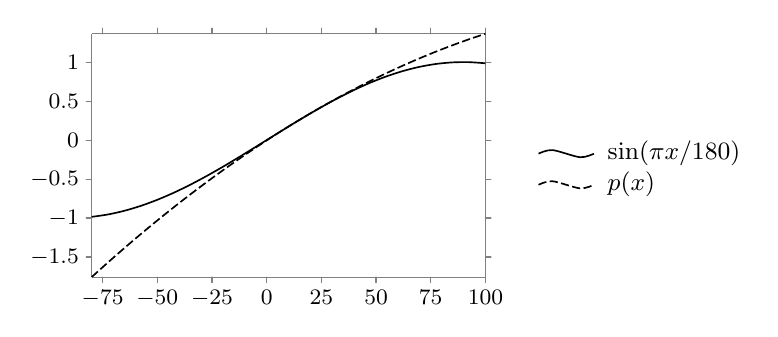
\begin{tikzpicture}
      \datavisualization [%
        scientific axes,
        visualize as smooth line/.list={sin, poly},
        legend=east outside,
        sin={label in legend={text=$\sin(\pi x / 180)$}},
        poly={label in legend={text=$p(x)$}},
        style sheet=vary dashing
      ]
      data [set=poly, format=function] {
        var x : interval [-80:100];
        func y = -0.00005 * (\value x)^2 + 0.01825 * (\value x) - 0.0039;
      }
      data [set=sin, format=function] {
        var x : interval [-80:100];
        func y = sin(pi * (\value x) / 180 r);
      };
    \end{tikzpicture}
    \caption{$\sin(\pi x/180)$と$p(x)$の比較}
  \end{figure}

  この近似の妥当性を考える.\cref{theorem:lagrange_error},および
  \[
    \abs*{\diff*[3]{\sin\pqty*{\frac{\pi}{180} x}}{x}} = \abs*{\pqty*{\frac{\pi}{180}}^3\cos\pqty*{\frac{\pi}{180} x}} \leqq \pqty*{\frac{\pi}{180}}^3
  \]
  により
  \[
    \abs*{\sin \degree{10.5} - p(10.5)} \leqq \pqty*{\frac{\pi}{180}}^3 \frac{1}{3!} \abs*{(12-10)}^3 \fallingdotseq 7.08\times 10^{-6}
  \]
  である.これは利用した近似値の有効数字である$4$桁よりも十分に小さいので,$\sin \degree{10.5} =  0.1822$は有効数字$4$桁で正しいと考えられる.
  実際,$\sin \degree{10.5} = 0.182236\dots$なので,確かに有効数字$4$桁で正しい値が得られている.
  また,有効数字$4$桁の数表に基づく限り,補間多項式の次数をこれ以上増やす必要は無いことも分かる.
\end{example}

\section{数値微分}
\subsection{数値微分}
関数を補間多項式で近似できるのなら,ある点における微分係数もまた,補間多項式の微分係数で近似できると考えられる.
すなわち,実数$x_1,\dots,x_n$はどの2つも相異なり,$t$が$x_1,\dots,x_n$に十分近いとき,
点$(x_1,f(x_1)),\dots,(x_n,f(x_n))$に関する補間多項式を$p(x)$とすると$f'(t) \fallingdotseq p'(t)$であると考えられる.

このような微分の近似を数値微分という.数値微分をするときは$x_1,\dots,x_n$を等間隔に取ることが多い.以下にこの場合の例を示す.

\begin{example}[数値微分の例1]
  \label{example:numerical_derivative_1}
  $n=2$かつ$(x_1,x_2)=(t,t+h)$のとき
  \[
    p(x) = f(t) + f[t,t+h](x-t)
  \]
  である.よって
  \[
    f'(t) \fallingdotseq {\diff{p}{x}}(t) = f[t,t+h] = \frac{f(t+h)-f(t)}{h}
  \]
  である.$h\to 0$においては,この式の右辺は厳密に$f'(t)$と等しくなる.
\end{example}

\begin{example}[数値微分の例2]
  \label{example:numerical_derivative_2}
  $n=3$かつ$(x_1,x_2,x_3)=(t-h,t,t+h)$のとき
  \[
    p(x) = f(t-h) + f[t-h,t]\pqty*{x-(t-h)} + f[t-h,t,t+h]\pqty*{x-(t-h)}(x-t)
  \]
  である.よって
  \begin{gather*}
    {\diff{p}{x}}(x) = f[t-h,t] + f[t-h,t,t+h](2x-2t+h) \\
    f'(t) \fallingdotseq \frac{f(t)-f(t-h)}{h} + \frac{h^{-1}\pqty*{f(t)-f(t-h)}-h^{-1}\pqty*{f(t+h)-f(t)}}{(t-h)-(t+h)}h
    = \frac{f(t+h)-f(t-h)}{2h}
  \end{gather*}
  である.この式についても,$h\to 0$においては
  \[
    \frac{f(t+h)-f(t-h)}{2h} = \frac{f(t+h)-f(t)}{2h} + \frac{f(t)-f(t-h)}{2h} \to \frac{f'(t)}{2} + \frac{f'(t)}{2} = f'(t)\plimas{h\to 0}
  \]
  が成立する.
\end{example}

\begin{figure}[H]
  \centering
  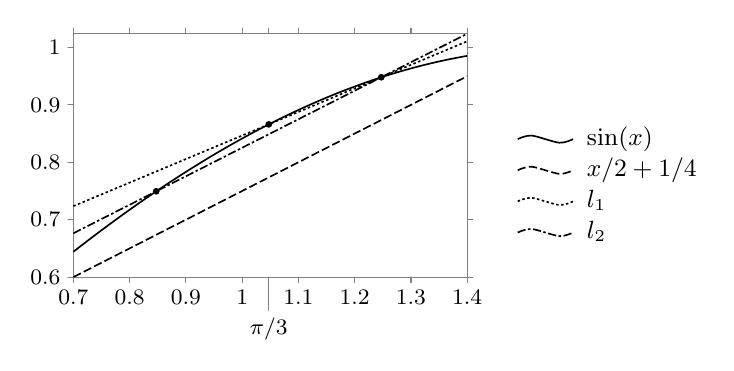
\begin{tikzpicture}
    \datavisualization [%
      scientific axes,
      visualize as smooth line/.list={sin, truth, deg1, deg2},
      visualize as scatter/.list={pts},
      legend=east outside,
      x axis={ticks={major also at={(pi/3) as [{tick text padding=1em}] $\pi/3$}}},
      pts={style={mark=*, mark size=1pt}},
      sin={label in legend={text=$\sin(x)$}},
      truth={label in legend={text=$x/2+1/4$}},
      deg1={label in legend={text=$l_1$}},
      deg2={label in legend={text=$l_2$}},
      style sheet=vary dashing
    ]
    data [set=sin, format=function] {
      var x : interval [0.7:1.4];
      func y = sin(\value x r);
    }
    data [set=truth, format=function] {
      var x : interval [0.7:1.4];
      func y = 0.5 * \value x + 0.25;
    }
    data [set=deg1, format=function] {
      var x : interval [0.7:1.4];
      func y = 0.436298 + 0.410359 * (\value x);
    }
    data [set=deg2, format=function] {
      var x : interval [0.7:1.4];
      func y = 0.328647 + 0.496673 * (\value x);
    }
    data [set=pts] {
      x, y
      0.847198, 0.749428
      1.0472, 0.866025
      1.2472, 0.948097
    };
  \end{tikzpicture}
  \caption{数値微分の比較}
\end{figure}

図は,2つの直線
\begin{align*}
  l_1 &\colon\, y = \frac{f(t+h)-f(t)}{h} (x - t) + f(t) \\
  l_2 &\colon\, y = \frac{f(t+h)-f(t-h)}{(t+h)-(t-h)} (x - (t-h)) + f(t-h)
\end{align*}
を$f(x)=\sin(x), t=\pi/3, h=0.2$の場合について示したものである.
図によれば,$l_2$は$l_1$よりも傾きが$1/2 = \cos(\pi/3)$に近い.
したがって,$(\sin(x))'$の$x=\pi/3$における近似に関しては,\cref{example:numerical_derivative_1}よりも\cref{example:numerical_derivative_2}のほうが真値に近い値を与えている.
より一般に,$h$を変えない場合,高次の補間多項式を利用した公式ほど近似値は真値に近づく傾向にある.

\section{数値積分}
\subsection{ニュートン・コーツの公式}
\label{subsection:newton_cotes}
関数$f(x)$の区間$I = [a, b]\,(a<b)$における定積分を考える.実数$x_1,\dots,x_n \in I$は$a \leqq x_1 < \dots < x_n \leqq b$を満たすとし,
点$(x_1,f(x_1)),\dots,(x_n,f(x_n))$に関する補間多項式を$p(x)$とおく.このとき,$p(x)$で$f(x)$がよく近似できていれば
\[
  \int_a^b f(x) \dd{x} \fallingdotseq \int_a^b p(x) \dd{x}
\]
となることが期待できる.

右辺について,\cref{definition:lagrange}の式を利用すると
\[
  \int_a^b p(x) \dd{x}
  = \int_a^b \pqty*{\sum_{i=1}^n f(x_i) \prod_{k\neq i} \frac{x - x_k}{x_i - x_k}} \dd{x}
  = \sum_{i=1}^n f(x_i) \int_a^b \prod_{k\neq i} \frac{x - x_k}{x_i - x_k} \dd{x}
\]
である.よって
\[
  w_i = \int_a^b \prod_{k\neq i} \frac{x - x_k}{x_i - x_k} \dd{x} \quad (i=1,\dots,n)
\]
とおくと,冒頭の近似式は
\[
  \int_a^b f(x) \dd{x} \fallingdotseq \sum_{i=1}^n w_i f(x_i)
\]
という形に書ける.

点$x_1,\dots,x_n$のことを標本点,実数$w_1,\dots,w_n$のことを重みという.
上の式から,重み$w_1,\dots,w_n$は積分区間$I$と標本点$x_1,\dots,x_n$の取り方のみに依存し,関数$f(x)$によらないことが分かる.

特にここで,実数$x_1,\dots,x_n$を区間$[a,b]$上で均等に取り
\[
  x_i = a + (b-a)\frac{i-1}{n-1} \quad (i = 1,\dots,n)
\]
として定積分を近似する方法を閉じたニュートン・コーツの公式という.
\footnote{端点を含めず,$x_i = a + (b-a)i/(n+1)$とする方法を開いたニュートン・コーツの公式という.性質は閉じたニュートン・コーツの公式とほとんど同様である.}

閉じたニュートン・コーツの公式の誤差は,\cref{theorem:lagrange_error}の不等式を両辺ともに積分することで評価できる.
実際
\begin{align*}
  \abs*{\int_a^b f(x) \dd{x} - \int_a^b p(x) \dd{x}}
  &\leqq \int_a^b \abs*{f(x) - p(x)} \dd{x} \\
  &\leqq (b-a)\max_{a\leqq t\leqq b} \abs*{f(t) - p(t)} \\
  &\leqq (b-a)\pqty*{\max_{a\leqq\xi\leqq b} \frac{\abs*{f^{(n)}(\xi)}}{n!} (b-a)^n} \\
  &= \max_{a\leqq\xi\leqq b} \frac{\abs*{f^{(n)}(\xi)}}{n!} (b-a)^{n+1}
\end{align*}
である(ただし,この評価は最良ではない.ニュートン・コーツの公式に関しては,より良い評価方法が知られている).

以下では$n=2,3$について,$w_1,\dots,w_n$を計算し誤差を見積もる.

\begin{example}[台計則]
  $n=2$のとき
  \begin{align*}
    w_1
    &= \int_a^b \frac{x-x_2}{x_1-x_2} \dd{x}
     = \int_a^b \frac{x-b}{a-b} \dd{x}
     = \frac{b-a}{2} \\
    w_2
    &= \int_a^b \frac{x-x_1}{x_2-x_1} \dd{x}
     = \int_a^b \frac{x-a}{b-a} \dd{x}
     = \frac{b-a}{2}
  \end{align*}
  である.つまり,$n=2$のときの閉じたニュートン・コーツの公式は
  \[
    \int_a^b f(x) \dd{x} \fallingdotseq \frac{b-a}{2} \pqty*{f(a)+f(b)}
  \]
  と表される.この公式を台計則という.台計則の誤差は
  \[
    \abs*{\int_a^b f(x) \dd{x} - \int_a^b p(x) \dd{x}}
    \leqq \max_{a\leqq\xi\leqq b} \frac{\abs*{f^{(2)}(\xi)}}{2} (b-a)^3
  \]
  と評価できる.なお,台計則は2点$(a,f(a)),(b,f(b))$に関する補間多項式を利用しているので,$1$次以下の多項式関数に関しては(\cref{theorem:interpolation}により)厳密な値を与える.

  なお,本稿では示さないが,もう少し厳しく
  \[
    \abs*{\int_a^b f(x) \dd{x} - \int_a^b p(x) \dd{x}} \leqq \max_{a\leqq\xi\leqq b} \frac{\abs*{f^{(2)}(\xi)}}{12} (b-a)^3
  \]
  と評価できることが知られている\cite{kikuchi}.
\end{example}

\begin{example}[シンプソン則]
  $n=3$のとき
  \begin{align*}
    w_1
    &= \int_a^b \frac{(x-x_2)(x-x_3)}{(x_1-x_2)(x_1-x_3)} \dd{x}
     = \int_a^b \frac{\pqty*{x-2^{-1}(a+b)}(x-b)}{\pqty*{a-2^{-1}(a+b)}(a-b)} \dd{x}
     = \frac{b-a}{6} \\
    w_2
    &= \int_a^b \frac{(x-x_1)(x-x_3)}{(x_2-x_1)(x_2-x_3)} \dd{x}
     = \int_a^b \frac{(x-a)(x-b)}{\pqty*{2^{-1}(a+b)-a}\pqty*{2^{-1}(a+b)-b}} \dd{x}
     = \frac{2(b-a)}{3} \\
    w_3
    &= \int_a^b \frac{(x-x_1)(x-x_2)}{(x_3-x_1)(x_3-x_2)} \dd{x}
     = \int_a^b \frac{(x-a)(x-2^{-1}(a+b))}{(b-a)(b-2^{-1}(a+b))} \dd{x}
     = \frac{b-a}{6}
  \end{align*}
  である.つまり,$n=3$のときの閉じたニュートン・コーツの公式は
  \[
    \int_a^b f(x) \dd{x} \fallingdotseq \frac{b-a}{6}\pqty*{f(a) + 4f\pqty*{\frac{a+b}{2}} + f(b)}
  \]
  と表される.この公式をシンプソン則という.シンプソン則の誤差は
  \[
    \abs*{\int_a^b f(x) \dd{x} - \int_a^b p(x) \dd{x}}
    \leqq \max_{a\leqq\xi\leqq b} \frac{\abs*{f^{(3)}(\xi)}}{6} (b-a)^4
  \]
  と評価できる.

  台計則と同様に考えれば,シンプソン則は$2$次以下の多項式関数について厳密な値を与えることが分かる.
  ところが,シンプソン則はさらに性質が良い.$f(x)=x^3$のときを考えると,このとき
  \[
    \frac{b-a}{6}\pqty*{f(a) + 4f\pqty*{\frac{a+b}{2}} + f(b)}
    = \frac{b-a}{6}\pqty*{a^3 + 4\pqty*{\frac{a+b}{2}}^3 + b^3}
    = \frac{b^4-a^4}{4}
    = \int_a^b f(x) \dd{x}
  \]
  である.つまり,シンプソン則は$3$次多項式関数についても厳密な値を与える.

  実は,シンプソン則の誤差は
  \[
    \abs*{\int_a^b f(x) \dd{x} - \int_a^b p(x) \dd{x}} \leqq \max_{a\leqq\xi\leqq b} \frac{\abs*{f^{(4)}(\xi)}}{2880} (b-a)^5
  \]
  と評価できることが知られている\cite{kikuchi}.この式からも,シンプソン則が$3$次以下の多項式関数について厳密な値を与えることが分かる.
\end{example}

\begin{example}[台形則とシンプソン則の比較]
  \label{example:simpson_vs_trapezoid}
  \begin{figure}[H]
    \centering
    \begin{tikzpicture}
      \datavisualization [%
        scientific axes,
        visualize as smooth line/.list={exp, deg1, deg2},
        legend=east outside,
        exp={label in legend={text=$e^x$}},
        deg1={label in legend={text={台形則}}},
        deg2={label in legend={text={シンプソン則}}},
        style sheet=vary dashing
      ]
      data [set=exp, format=function] {
        var x : interval [-3:1];
        func y = exp(\value x);
      }
      data [set=deg1, format=function] {
        var x : interval [-3:1];
        func y = (exp(1)-exp(-3)) * (\value x - 1) / 4 + e;
      }
      data [set=deg2, format=function] {
        var x : interval [-3:1];
        func y = (e/8 - 1/(4*e) + 1/(8*e^3)) * (\value x)^2 + (e/2 - 1/(2*e)) * (\value x) + 3*e/8 + 3/(4*e) - 1/(8*e^3);
      };
    \end{tikzpicture}
    \caption{台形則とシンプソン則}
  \end{figure}
  
  図は,定積分$\displaystyle \int_{-3}^1 e^x \dd{x}$の台形則とシンプソン則による近似で利用される補間多項式を示したものである.
  この場合,シンプソン則では$e^x$の下側を通る部分と上側を通る部分がちょうど相殺され,より真値に近い値が得られると期待できる.
  実際,この真値は
  \[
    \int_{-3}^1 e^x \dd{x} = 2.6685\dots
  \]
  であり,台形則とシンプソン則による近似値はそれぞれ
  \begin{align*}
    \frac{1-(-3)}{2} \pqty*{e^{-3}+e^1} &= 5.5361\dots \\
    \frac{1-(-3)}{6} \pqty*{e^{-3} + 4e^{-1} + e^1} &= 2.8263\dots
  \end{align*}
  である.  
\end{example}

閉じたニュートン・コーツの公式はたいてい,積分区間を複数の小区間に区切ってから,その各区間に対して適用される.
この場合,台計則は複合台計則,シンプソン則は複合シンプソン則と呼ばれる(単に台形則,シンプソン則とも呼ばれる).
例で見たように,閉じたニュートン・コーツの公式の誤差は$b-a$に依存する.したがって,複合台形公式と複合シンプソン則の誤差は,$b-a$を小さく取るほど,
すなわち,区間を多く分割するほど改良されると考えられる.

\subsection{ガウス・ルジャンドル公式}
ニュートン・コーツの公式では標本点を均等に取って定積分を近似した.
この節では,標本点の取り方を工夫することで,ニュートン・コーツの公式と比べて少ない標本点で良い近似を得る方法を示す.

\begin{definition}{ルジャンドル多項式}{legendre_polynomial}
  正の整数$n$に対し
  \[
    L_n(x) = \frac{1}{2^n n!} \diff*[n]{\bqty*{(x^2 -1)^n}}{x}
  \]
  で定義される多項式を$n$次のルジャンドル多項式という{\footnotemark}.
\end{definition}
\footnotetext{正確には,この式における$\diff {}/x$は形式微分である.本稿では普通の微分と特に区別せず扱う.}

\begin{example}[ルジャンドル多項式の例]
  \begin{align*}
    L_1(x) &= \frac{1}{2} \cdot 2x = x
      & L_2(x) &= \frac{1}{8} (12x^2-4) = \frac{1}{2} (3x^2 - 1) & \\
    L_3(x) &= \frac{1}{48} (120 x^3 - 72x) = \frac{1}{2} (5x^3 - 3x)
      & L_4(x) &= \frac{1}{8} (63x^5-70x^3+15x)
  \end{align*}
  である.
\end{example}

\begin{figure}[H]
  \centering
  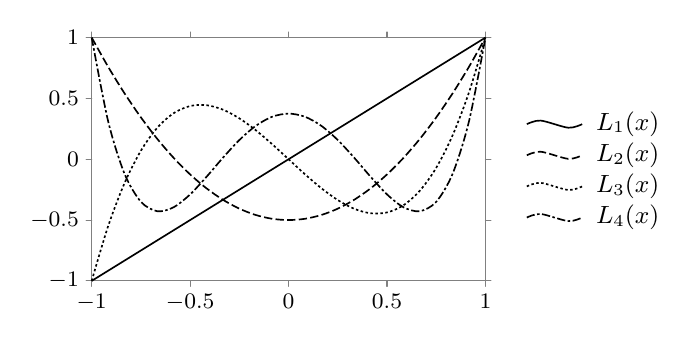
\begin{tikzpicture}
    \datavisualization [%
      scientific axes,
      x axis={ticks=few},
      visualize as smooth line/.list={deg1, deg2, deg3, deg4},
      legend=east outside,
      deg1={label in legend={text=$L_1(x)$}},
      deg2={label in legend={text=$L_2(x)$}},
      deg3={label in legend={text=$L_3(x)$}},
      deg4={label in legend={text=$L_4(x)$}},
      style sheet=vary dashing
    ]
    data [set=deg1, format=function] {
      var x : interval [-1:1];
      func y = \value x;
    }
    data [set=deg2, format=function] {
      var x : interval [-1:1];
      func y = 0.5 * (3*(\value x)^2 - 1);
    }
    data [set=deg3, format=function] {
      var x : interval [-1:1];
      func y = 0.5 * (5*(\value x)^3 - 3*(\value x));
    }
    data [set=deg4, format=function] {
      var x : interval [-1:1];
      func y = (1/8) * (35*(\value x)^4 - 30*(\value x)^2 + 3);
    };
  \end{tikzpicture}
  \caption{$n=1,2,3,4$のときのルジャンドル多項式$L_n(x)$}
\end{figure}

\begin{theorem}{}{legendre_polynomial_root}
  $L_n(x)$は区間$\mathring{I} = (-1,1)$に$n$個の相異なる根{\footnotemark}を持つ.
\end{theorem}
\footnotetext{多項式$f(x)$の根とは$f(\alpha)=0$を満たす値$\alpha$のことである.}

この定理を示す前に,次の補題を示す.

\begin{lemma}{一般ライプニッツ則}{leibniz}
  関数$f(x), g(x)$は$n$階微分可能とする.このとき,正の整数$n$に対して
  \[
    \diff*[n]{\pqty*{f(x)g(x)}}{x} = \sum_{k=0}^n \binom{n}{k} f^{(k)}(x) g^{(n-k)}(x)
  \]
  である.ただし$\binom{n}{k}$は二項係数である.
\end{lemma}

\begin{proof}
  帰納法により示す.$n=1$のとき,積の微分法則により
  \[
    \diff*{\pqty*{f(x)g(x)}}{x} = f(x)g'(x) + f'(x)g(x)
  \]
  であり成り立つ.また,ある$n$での成立を仮定すると
  \begin{align*}
    \diff*[n+1]{\pqty*{f(x)g(x)}}{x}
    &= \diff*{\pqty*{\diff*[n]{f(x)g(x)}{x}}}{x} \\
    &= \diff*{\sum_{k=0}^n \binom{n}{k} f^{(k)}(x) g^{(n-k)}(x)}{x} \\
    &= \sum_{k=0}^n \binom{n}{k} \pqty*{f^{(k)}(x) g^{(n-k+1)}(x) + f^{(k+1)}(x) g^{(n-k)}(x)} \\
    &= \sum_{k=0}^{n} \binom{n}{k} f^{(k)}(x) g^{(n+1-k)}(x) + \sum_{k=1}^{n+1} \binom{n}{k-1} f^{((k-1)+1)}(x) g^{(n-(k-1))}(x) \\
    &= f(x)g^{(n+1)}(x) + \pqty*{\sum_{k=1}^{n} \pqty*{\binom{n}{k} + \binom{n}{k-1}} f^{(k)}(x) g^{(n+1-k)}(x)} + f^{(n+1)}(x)g(x) \\
    &= \sum_{k=0}^{n+1} \binom{n+1}{k} f^{(k)}(x) g^{(n+1-k)}(x) \quad \pqty*{\because\, \binom{n}{k} + \binom{n}{k-1} = \binom{n+1}{k}}
  \end{align*}
  となり,成立が確かめられる.
\end{proof}

\cref{lemma:leibniz}により,\cref{theorem:legendre_polynomial_root}は以下のように証明できる.

\begin{proof}
  $x^n$を$k$階微分したときの係数を$A_k$とする.
  \[
    f(x) = \pqty*{x^2-1}^n = (x-1)^n (x+1)^n
  \]
  とおく.\cref{lemma:leibniz}により,$l=1,\dots,n-1$について
  \begin{align*}
    f^{(l)}(x)
    &= \sum_{k=0}^l \binom{l}{k} \pqty*{\diff*[k]{(x-1)^n}{x}} \pqty*{\diff*[l-k]{(x+1)^n}{x}} \\
    &= \sum_{k=0}^l \binom{l}{k} A_{k} (x-1)^{n-k} A_{l-k} (x+1)^{n-(l-k)} \\
    &= (x-1)^{n-l} (x+1)^{n-l} \sum_{k=0}^l \binom{l}{k} A_{k} A_{l-k} (x-1)^{l-k} (x+1)^k
  \end{align*}
  である.よって,$f^{(1)}(x),\dots,f^{(n-1)}(x)$の$x=-1,1$における値は$0$である.

  このことを用い,$l=1,\dots,n$について$f^{(l)}(x)$が区間$\mathring{I}$上に$l$個の相異なる根を持つことを示す.
  まず,$l=1$のときは平均値の定理により
  \[
    f'(\xi) = \frac{f(1)-f(-1)}{1-(-1)} = \frac{0-0}{1-(-1)}=0
  \]
  を満たす$\xi \in \mathring{I}$が存在する.

  次に,ある$l<n$での成立を仮定する.すなわち,$l$個の実数$\xi_1, \dots, \xi_l \in \mathring{I}$(ただし$\xi_1 < \cdots < \xi_l$とする)が存在して,$f^{(l)}(\xi_1) = \cdots = f^{(l)}(\xi_l) = 0$を満たすとする.
  このとき,$\xi_0 = -1, \xi_{l+1} = 1$とおくと,平均値の定理により$k=0,\dots,l$に対し
  \[
    f^{(l+1)}(\xi'_k) = \frac{f^{(l)}(\xi_k) - f^{(l)}(\xi_{k+1})}{\xi_k - \xi_{k+1}} = \frac{0 - 0}{\xi_k - \xi_{k+1}} = 0
  \]
  を満たす$\xi'_k \in (\xi_k, \xi_{k+1}) \subset \mathring{I}$が存在する.
  よって,$f^{(l+1)}(x)$もまた$l+1$個の相異なる根を$\mathring{I}$上に持つ.

  以上により,帰納的に$f^{(n)}(x)$は$\mathring{I}$上に$n$個の相異なる根を持つ.
  $2^n n! L_n(x) = f^{(n)}(x)$なので,$L_n(x)$もまた$\mathring{I}$上に$n$個の相異なる根を持つ.
\end{proof}

\begin{theorem}{}{orthogonality}
  $k = 1,\dots,n-1$なら
  \[
    \int_{-1}^1 x^k L_n(x) \dd{x} = 0
  \]
  である.
\end{theorem}

\begin{proof}
  \cref{theorem:legendre_polynomial_root}の証明と同様に
  \[
    f(x) = \pqty*{x^2-1}^n = (x-1)^n (x+1)^n
  \]
  とおく.このとき
  \[
    \int_{-1}^1 x^k L_n(x) \dd{x}
    = \int_{-1}^1 x^k \frac{1}{2^n n!} f^{(n)}(x) \dd{x}
    = \frac{1}{2^n n!} \int_{-1}^1 x^k f^{(n)}(x) \dd{x}
  \]
  である.部分積分により
  \[
    \int_{-1}^1 x^k f^{(n)}(x) \dd{x}
    = \bqty*{x^k f^{(n-1)}(x)}_{-1}^1 - \int_{-1}^1 kx^{k-1} f^{(n-1)}(x) \dd{x}
  \]
  であるが,\cref{theorem:legendre_polynomial_root}の証明で見たように,$l=1,\dots,n-1$に対して
  \[
    f^{(l)}(-1) = f^{(l)}(1) = 0
  \]
  なので
  \[
    \int_{-1}^1 x^k f^{(n)}(x) \dd{x}
    = -k\int_{-1}^1 x^{k-1} f^{(n-1)}(x) \dd{x}
  \]
  である.同様に部分積分を繰り返すことで
  \[
    \abs*{\int_{-1}^1 x^k f^{(n)}(x) \dd{x}}
    = \abs*{\int_{-1}^1 k! x^0 f^{(n-k)}(x) \dd{x}}
    = k! \abs*{f^{(n-k-1)}(1) - f^{(n-k-1)}(-1)}
    = 0
  \]
  が得られる.よって
  \[
    \int_{-1}^1 x^k L_n(x) \dd{x}
    = \frac{1}{2^n n!} \int_{-1}^1 x^k f^{(n)}(x) \dd{x}
    = 0
  \]
  である.
\end{proof}

以上により,次の定理がしたがう.

\begin{theorem}{ガウス・ルジャンドル公式}{gauss_legendre}
  $\mathring{I} = (-1,1)$とし,$x_1,\dots,x_n$を$\mathring{I}$上にある$L_n(x)$の相異なる$n$個の根とする.
  このとき,$f(x)$が$2n-1$次以下の多項式関数であれば,点$(x_1,f(x_1)),\dots,(x_n,f(x_n))$に関する補間多項式$p(x)$は
  \[
    \int_{-1}^1 f(x) \dd{x} = \int_{-1}^1 p(x) \dd{x}
  \]
  を満たす.言い換えると,重み$w_1,\dots,w_n$を
  \[
    w_i = \int_a^b \prod_{k\neq i} \frac{x - x_k}{x_i - x_k} \dd{x}
    \quad (i = 1,\dots,n)
  \]
  で定めると
  \[
    \int_{-1}^1 f(x) \dd{x} = \sum_{i=1}^n w_i f(x_i)
  \]
  が成り立つ.
\end{theorem}

\begin{proof}
  $L_n(x)$の相異なる$n$個の根を$x_1,\dots,x_n$とおく.
  関数$f(x)$に対し
  \[
    G[f(x)] = \sum_{i=1}^n w_i f(x_i),
    \quad w_i = \int_a^b \prod_{k\neq i} \frac{x - x_k}{x_i - x_k} \dd{x}
  \]
  とする\footnote{本来は$G[f]$と書くべきであろうが,本稿では分かりやすさを優先した.}.
  \cref{subsection:newton_cotes}で見たように,$G[f(x)]$は点$(x_1,f(x_1)),\dots,(x_n,f(x_n))$に関する補間多項式を区間$[-1, 1]$で定積分した値である.

  $G[\cdot]$の定義により,$I$で定義される任意の関数$f(x), g(x)$に関して
  \[
    G[f(x) + g(x)] = G[f(x)] + G[g(x)]
  \]
  が成立する.

  $f(x)$を$2n-1$次以下の多項式関数とすると,$f(x)$は(多項式の意味で)$L_n(x)$により割れる.商を$q(x)$,余りを$r(x)$とすると
  \[
    f(x) = q(x)L_n(x) + r(x)
  \]
  となる.したがって
  \[
    G[f(x)] = G[q(x)L_n(x)] + G[r(x)]
  \]
  であるが,$x_1,\dots,x_n$は$L_n(x)$の根であるから
  \[
    G[q(x)L_n(x)]
    = \sum_{k=1}^n w_k q(x_k) L_n(x_k)
    = \sum_{k=1}^n w_k q(x_k) \cdot 0
    = 0
  \]
  である.
  したがって$G[f(x)] = G[r(x)]$である.
  $r(x)$の次数は$L_n(x)$の次数を超えないので,$r(x)$の次数は最大でも$n-1$である.
  よって,\cref{theorem:interpolation}により点$(x_1,r(x_1)),\dots,(x_n,r(x_n))$に関する補間多項式は$r(x)$に一致する.
  すなわち
  \[
    G[f(x)] = G[r(x)] = \int_{-1}^1 r(x) \dd{x}
  \]
  である.

  一方,$q(x)$の次数は$n-1$以下なので,\cref{theorem:orthogonality}により
  \[
    \int_{-1}^1 f(x) \dd{x}
    = \int_{-1}^1 q(x)L_n(x) \dd{x} + \int_{-1}^1 r(x) \dd{x}
    = \int_{-1}^1 r(x) \dd{x}
  \]
  である.よって
  \[
    G[f(x)] = \int_{-1}^1 r(x) \dd{x} = \int_{-1}^1 f(x) \dd{x}
  \]
  が成り立つ.
\end{proof}

\cref{theorem:gauss_legendre}により,関数$f(x)$が$2n-1$次以下の多項式関数でよく近似できるときは,
標本点をルジャンドル多項式$L_n(x)$の$n$個の根にすることで,より正確な近似値が得られると考えられる.この方法をガウス・ルジャンドル公式という.

\begin{example}[ガウス・ルジャンドル公式とシンプソン則の比較]
  定積分$\displaystyle \int_{-3}^1 e^x \dd{x}$をガウス・ルジャンドル公式によって近似する.

  定積分$\displaystyle \int_{-3}^1 e^x \dd{x}$は積分区間が$[-1, 1]$でない.そこで,置換積分により変数を
  \[
    t = \frac{x+1}{2},\, \dd{x} = 2\dd{t}
  \]
  に変え$\displaystyle \int_{-1}^1 2e^{2t-1} \dd{t}$を計算する.
  $L_3(x)$の根$x_1,x_2,x_3\,(x_1<x_2<x_3)$は,方程式$L_3(x)=0$を解くことで
  \[
    \frac{1}{2} (5x^3 - 3x) = 0 \quad\therefore\,
    x_1 = -\sqrt{\frac{3}{5}}, x_2 = 0, x_3 = \sqrt{\frac{3}{5}}
  \]
  と分かる.$x_1,x_2,x_3$に対応する重みはそれぞれ
  \[
    w_1 = \frac{5}{9}, w_2 = \frac{8}{9}, w_3 = \frac{5}{9}
  \]
  である.したがって,ガウス・ルジャンドル公式によれば$f(x)=2e^{2x-1}$とすると
  \[
    \int_{-1}^1 2e^{2t-1} \dd{t}
    \fallingdotseq \frac{5}{9}f\pqty*{-\sqrt{\frac{3}{5}}} + \frac{8}{9}f\pqty*{0} + \frac{5}{9}f\pqty*{\sqrt{\frac{3}{5}}}
    = 2.6651\dots
  \]
  である.これは\cref{example:simpson_vs_trapezoid}で見たシンプソン則による近似値$2.8263\dots$よりも真値$2.6685\dots$に近い.
\end{example}

\section{補遺}
\subsection{ルンゲ現象}
\cref{theorem:lagrange_error}の状況で,$f(x)=(25x^2+1)^{-1}$のときを考える.
\[
  x_i = -1 + 2\cdot\frac{i-1}{n-1} \quad (i=1,\dots,n)
\]
とおき,$p_n(x)$を点$(x_1, f(x_1)),\dots,(x_n,f(x_n))$に関する補間多項式としたとき,
その様子は下図のようになる.

\begin{figure}[H]
  \centering
  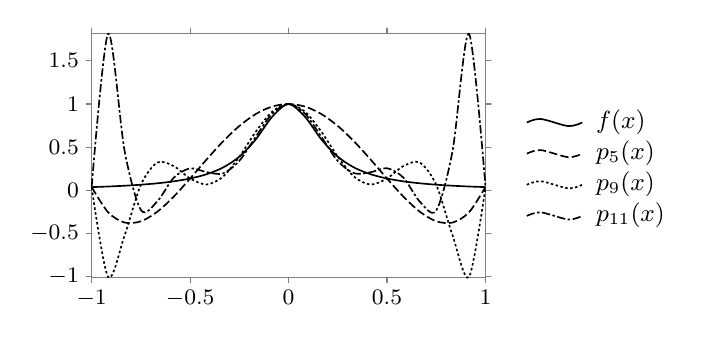
\begin{tikzpicture}
    \datavisualization [%
      scientific axes,
      x axis={ticks=few},
      visualize as smooth line/.list={func, deg4, deg8 ,deg10},
      legend=east outside,
      func={label in legend={text=$f(x)$}},
      deg4={label in legend={text=$p_5(x)$}},
      deg8={label in legend={text=$p_9(x)$}},
      deg10={label in legend={text=$p_{11}(x)$}},
      style sheet=vary dashing
    ]
    data [set=func, format=function] {
      var x : interval [-1:1];
      func y = 1 / (25*(\value x)^2 + 1);
    }
    data [set=deg4, format=function] {
      var x : interval [-1:1];
      func y = 3.3156 * (\value x)^4 - 4.2772 * (\value x)^2 + 1;
    }
    data [set=deg8, format=function] {
      var x : interval [-1:1];
      func y = 53.689 * (\value x)^8 - 102.82 * (\value x)^6 + 61.367 * (\value x)^4 - 13.203 * (\value x)^2 + 1;
    }
    data [set=deg10, format=function] {
      var x : interval [-1:1];
      func y = -220.94 * (\value x)^10 + 494.91 * (\value x)^8 - 381.43 * (\value x)^6 + 123.36 * (\value x)^4 - 16.855 * (\value x)^2 + 1;
    };
  \end{tikzpicture}
  \caption{$f(x)$と$n=5,9,11$のときの$p_n(x)$}
\end{figure}

図によれば,補間多項式が通るべき点の個数$n$を増やすほど,$p_n(x)$は$f(x)$からかけ離れている.その様子は特に$x=\pm 1$付近で顕著である.
このような現象をルンゲ現象という.

ルンゲ現象により,ニュートン・コーツの公式においてただ次数を増やしても,積分の近似値は改良されないと考えられる.
複合台形則,複合シンプソン則などが利用されるのはこのためである.

ルンゲ現象を回避するには,補間多項式が通るべき点の$x$座標をチェビシェフノード
\[
  x_i = \cos\pqty*{\frac{2i-1}{2n} \pi}\quad (i = 1, \dots, n)
\]
にすると良いことが知られている\cite{horinouchi}.このとき,$n=9$の下で補間多項式$p(x)$は下図のようになる.
確かに$x=\pm 1$付近における振動が抑制されていることが分かる.

\begin{figure}[H]
  \centering
  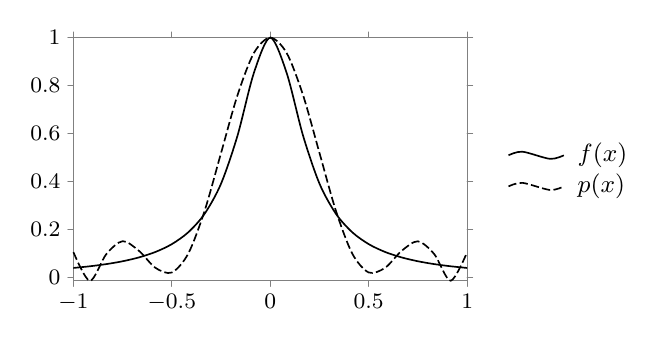
\begin{tikzpicture}
    \datavisualization [%
      scientific axes,
      x axis={ticks=few},
      visualize as smooth line/.list={func, deg8},
      legend=east outside,
      func={label in legend={text=$f(x)$}},
      deg8={label in legend={text=$p(x)$}},
      style sheet=vary dashing
    ]
    data [set=func, format=function] {
      var x : interval [-1:1];
      func y = 1 / (25*(\value x)^2 + 1);
    }
    data [set=deg8, format=function] {
      var x : interval [-1:1];
      func y = 17.6203 * (\value x)^8 - 40.3505 * (\value x)^6 + 31.3483 * (\value x)^4 - 9.51344 * (\value x)^2 + 1;
    };
  \end{tikzpicture}
  \caption{チェビシェフノードを利用した補間多項式}
\end{figure}

\subsection{補間多項式とテイラー多項式の関係}
この節では,補間多項式がテイラー多項式の近似と見なせることを述べる.

点$t$のまわりで$n$階微分可能な関数$f(x)$に対して,次の多項式を$n$次のテイラー多項式という.
\[
  p_n(x)=\sum_{k=0}^n \frac{f^{(k)}(t)}{k!} (x-t)^k=f(t)+f'(t)(x-t)+\cdots+\frac{f^{(n)}(t)}{n!} (x-t)^n
\]

関数$f(x)$が点$t$のまわりでテイラー展開可能であるとは,定義域における任意の$x$で
\[
  f(x)=\lim_{n\to\infty} p_n(x)=\sum_{n=0}^\infty\frac{f^{(n)}(t)}{n!} (x-t)^n
\]
が成立することをいい,この級数で元の関数を表現することをテイラー展開という.

一般には,関数が何回でも微分可能であってもテイラー展開可能とは限らない.しかし,実用上よく表れる関数はしばしばテイラー展開可能である.
たとえば,関数$\cos x,\sin x,e^x$は定義域における任意の点でテイラー展開可能である.

まず$n=2$のときについて考える.$2$次のテイラー多項式
\[
  p_2(x)=f(t)+f'(t)(x-t)+\frac{f''(t)}{2}(x-t)^2
\]
について,この式に表れる微分係数を
\[
  f'(t)\fallingdotseq\frac{f(t+h)-f(t)}{h},\quad f''(t)\fallingdotseq\frac{\pqty*{f(t+h)-f(t)}h^{-1}-\pqty*{f(t)-f(t-h)}h^{-1}}{h}
\]
のように,十分小さな$h$で近似することを考える.この近似は次のように書き換えられる.
\[
  f'(t)\fallingdotseq f[t+h,t],\quad f''(t)\fallingdotseq 2\cdot\frac{f[t+h,t]-f[t,t-h]}{(t+h)-(t-h)}=2f[t+h,t,t-h]
\]

すると,これを$p_2(x)$に代入すれば
\[
  p_2(x)\fallingdotseq f(t)+f[t,t-h](x-t)+f[t+h,t,t-h](x-t)^2
\]
となり,さらに,$h$が十分小さければ$x-(t+h)\fallingdotseq x-t$であるので
\[
  p_2(x)\fallingdotseq f(t)+f[t+h,t](x-(t+h))+f[t+h,t,t-h](x-(t+h))(x-t)
\]
である.\cref{theorem:newton}により,右辺は点$(t-h,f(t-h)),(t,f(t)),(t+h,f(t+h))$に関する補間多項式である.

以下では一般の$n$についても,補間多項式がテイラー多項式の近似と見なせることを示す.

\begin{theorem}{差商に対する平均値の定理}{divdif_mean}
  実数$x_1,\dots,x_{n+1}$はどの2つも相異なるとし,$x_1,\dots,x_{n+1}$の中で最小のものを$m$,最大のものを$M$とおく.
  また,関数$f(x)$は区間$I = [m, M]$で$n$階微分可能であるとする.
  このとき,次式を満たす$\xi \in (m, M)$が存在する.
  \[
    f[x_1,\dots,x_{n+1}] = \frac{f^{(n)}(\xi)}{n!}
  \]
\end{theorem}

\begin{proof}
  点$(x_1,f(x_1)),\dots,(x_{n+1},f(x_{n+1}))$に関する補間多項式を$p(x)$とおくと,
  関数$g(x)=f(x)-p(x)$は$x_1,\dots,x_{n+1}$を零点\footnote{関数$f(x)$の零点とは$f(\alpha)=0$を満たす値$\alpha$のことである.}に持つ.
  したがって,\cref{lemma:zero_existance}により$g^{(n)}(\xi)=0$を満たす$\xi\in (m, M)$が存在する.
  ここで,$p(x)$は\cref{theorem:newton}により
  \[
    p(x) = f(x_1) + \sum_{k=1}^{n} f[x_1,\dots,x_{k+1}] (x-x_1) \cdots (x-x_k)
  \]
  と表せる.よって$p^{(n)}(x) = f[x_1,\dots,x_{n+1}]n!$であり
  \[
    f^{(n)}(\xi) - f[x_1,\dots,x_{n+1}]n! = 0
    \quad\therefore\,
    f[x_1,\dots,x_{n+1}] = \frac{f^{(n)}(\xi)}{n!}
  \]
  が成立する.
\end{proof}

関数$f(x)$はある開区間$\mathring{I}$で$n$階微分可能かつ,$n$次導関数$f^{(n)}(x)$は$\mathring{I}$で連続とする.
$t=x_{n+1}\in\mathring{I}$をある定数とし,実数$s=x_1\in\mathring{I}$は$s<t$を満たすとする.$J=[s,t]$とおく.
$n$個の実数$x_1,\dots,x_n \in J$はすべて$s$の関数であり,任意の$s$について$x_1,\dots,x_{n+1}$はどの2つも相異なるものとする.

点$(x_1,f(x_1)),\dots,(x_{n+1},f(x_{n+1}))$に関する補間多項式を$p(x)$とおくと,$p(x)$は
\[
  p(x) = f(x_1) + \sum_{k=1}^n f[x_1,\dots,x_{k+1}] (x-x_1) \cdots (x-x_k)
\]
と書ける.\cref{theorem:divdif_mean}により,各$f[x_1,\dots,x_{k+1}]$に対して
\[
  f[x_1,\dots,x_{k+1}] = \frac{f^{(k)}(\xi_k)}{k!}
\]
を満たす$\xi_k\in J$が存在する.

関数$f^{(k)}(x)$は閉区間$J$で連続なので,$J$における最小値$m_k$,最大値$M_k$が存在する.
また,$f^{(k)}(x)$は$\mathring{I}$で連続なので$m_k, M_k\to f^{(k)}(t)\plimas{s\to t-0}$である.よって,はさみうちの原理により
\[
  f[x_1,\dots,x_{k+1}] \to \frac{f^{(k)}(t)}{k!}\plimas{s\to t-0}
\]
が成り立つ.したがって,任意の実数$x$について
\[
  p(x)=f(x_1)+\sum_{k=1}^n f[x_1,\dots,x_{k+1}](x-x_1)\cdots (x-x_k)\to f(t)+ \sum_{k=1}^n \frac{f^{(k)}(t)}{k!} (x-t)^k \plimas{s\to t-0}
\]
である.これにより$p(x)\to p_n(x)\plimas{s\to t-0}$であるので,$s$と$t$が十分に近ければ$p(x)\fallingdotseq p_n(x)$であり,
補間多項式をテイラー多項式の近似と見なせることが確かめられた.

\bibliography{reference}
\nocite{*}
\bibliographystyle{jplain}

\section*{更新履歴}
\begin{enumerate}[align=left]
  \item[2021.03.31] 初版
  \item[2021.04.08] 補遺「補間多項式とテイラー多項式の関係」を追加
  \item[2021.05.11] 誤字・脱字を修正
  \item[2021.05.27] \LaTeX ソースの不備を修正
\end{enumerate}

\end{document}
